\documentclass[12pt, a4paper, lithuanian, final]{article}

\usepackage{hyperref}
\usepackage{graphicx}
\usepackage{float}
\usepackage{placeins}
\usepackage{gensymb}
\usepackage{xcolor}
\usepackage{listings}
\usepackage{amsmath}
\usepackage{textgreek}
\usepackage{mathtools}
\usepackage[obeyFinal]{easy-todo}
\usepackage[utf8]{inputenc}
\def\LTfontencoding{L7x}
\usepackage[\LTfontencoding]{fontenc}
\usepackage[lithuanian]{babel}
%\usepackage{times}

%\renewcommand{\sfdefault}{uhv}
%\renewcommand{\rmdefault}{utm}
%\renewcommand{\ttdefault}{ucr}

\usepackage{VUMIF}

%Kodo highlitinimo configas
\lstset{basicstyle=\ttfamily,
	showstringspaces=false,
	commentstyle=\color{red},
	keywordstyle=\color{blue}
	}


% Titulinio puslapio reikalai
\vumifdept{Programų sistemų katedra}
\vumifpaper{}
\title{Praktikos uždarojoje akcinėje bendrovėje "`Elektromotus"' ataskaita}
\author{
    4 kurso 1 grupės studentas \\
    Rytis Karpuška
}

\supervisor{Irus Grinis, doc.}
\date{Vilnius \\
	2014}


\begin{document}

%titulinis ir turinys
\maketitle

\vumifsectionnonum{Įvadas}


%Skyrius apie įmonę
\section{Apie UAB "`Elektromotus"'}

UAB "`Elektromotus"' 2010 metais įkurta trijų steigėjų: Gintauto Palucko, Mindaugo Milašausko ir Šarūno Šutavičiaus su tikslu realizuoti jų sukauptą patirtį elektromobilių valdymo sistemų kūrimo srityje.
Nuo to laiko, įmonė išaugo ir samdyti darbuotojai pilnai perėmė įmonės darbo krūvius.
Šiuo metu įmonėje yra per 15 darbuotojų, metinė apyvarta viršyja milijoną litų, bei vykdomas ne vienas naujas projektas, su tikslu, patobulinti, išleisti, sukurti naujas technologijas bei produktus.

Buvo sukurti ir išleisti keli produktai, bei patentai.


\subsection{Produktai}
\subsubsection{"`Emus BMS"' - Baterijų valdymo sistema}
"`Emus BMS"' yra pagrindinis ir seniausias įmonės produktas, įnešantis daugiausiai pajamų.

Tai yra valdymo sistema vidutinėms ir didelėms ličio jonų, ličio polimerų, ličio geležies fosfatų, nikelio-metalo hidratų ir kitoms baterijoms.

Sistemą sudaro trijų lygmenų hierarchinė struktūra:

\begin{figure}[H]
\begin{center}
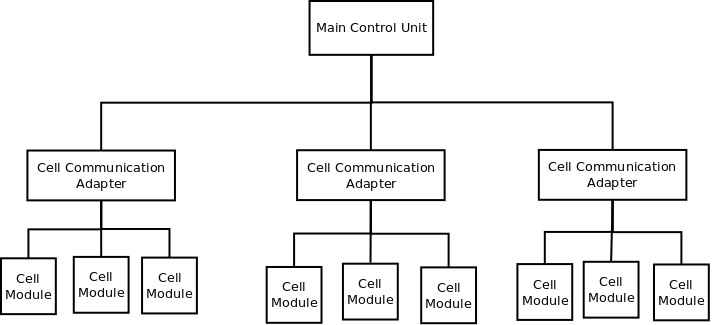
\includegraphics[width=1\textwidth]{img/bms_desc.png}
\caption{Emus BMS struktūra.}
\end{center}
\end{figure}

Sistemą sudaro šie komponentai:
\begin{itemize}
	\item{Main Control Unit} - Pagrindinis valdymo blokas, komunikuoja su komunikacijos adapteriais CAN sąsaja.
	\item{Cell Communication adapter} - Adapteris persiunčiantis CAN sąsajos komandas į celių modulius privačia įmonės sukurta sąsaja pritaikyta dirbti EMI triukšmingose sąlygose.
	\item{Cell module} - Celių moduliai, galiniai įrenginiai, matuoja celės įtampą, temperatūra, turi šiluminio balansavimo palaikymą.
\end{itemize}

Panašių sistemų rinkoje labai mažai, tad šį susilaukė populiarumo.
Ši sistema yra naudojama įvairiuose elektromobiliuose, laivuose, kranuose. ir t.t.

Ryškiausi klientų pasiekimai su "`Emus BMS"':
\begin{itemize}
	\item Komandos "`ACCIONA"' bolidas dalyvavęs "`Dakar"' ralyje
	\item Academic Motorsports Club Zurich (AMZ) automobilis, pasiekęs 100km/h per 1.785s, taip sumušdamas pasaulio rekordą
	\item "`Intersolar 2013, Munich"' saulės jegainės valdikliuose
	\item "`EcoPower Hybrid"' kranas dirbantis texaso uoste
	\item "`Lloyds paxter"' Pašto elektromobiliuose norvegijoje
\end{itemize}











%Skyrius apie mano veiklą įmonėje
\section{Veikla praktikos metu}

\subsection{Naujos Testavimo procedūros}

\subsubsection{"`Checker"' modulis}

\subsubsection{Regresiniai vienetų testai}








%Ko pasiekiau per tą laiką
\section{Rezultatai}


\subsection{Vidutinis klaidų paieškos laikas}

\subsection{Sugauti defektai regresinio vienetų testavimo metu}



\section{Išvados}

\bibliography{Bibliografija}
\begin{itemize}
	\item [[SM04]] - \textit{Taming the Embedded Tiger – Agile Test Techniques for Embedded Software}, \url{http://www.leanagilepartners.com/library/XR5_Taming_Embedded_Tiger.pdf}

\end{itemize}





\end{document}



